\documentclass{beamer} % "Beamer" is a word used in Germany to mean video projector. 

\usetheme{default} % Search online for beamer themes to find your favorite or use the Berkeley theme as in this file.

\usepackage{color} % It may be necessary to set PCTeX or whatever program you are using to output a .pdf instead of a .dvi file in order to see color on your screen.
\usepackage{graphicx} % This package is needed if you wish to include external image files.
\usepackage{tikz}

\title{3D Road Scene understanding with soft continuous occlusion modeling}
\author{Vikas Dhiman} 
\institute{NEC Laboratories America}
%\date{January 6, 2012} 


% 3D pose of the cars and ego motion
\newcommand{\pos}[2]{\mathbf{p}^{(#1)}(#2)}
\newcommand{\ori}[2]{\mathbf{\omega}^{(#1)}(#2)}
\newcommand{\state}[2]{\mathbf{s}^{#1}(#2)}

% ego pose
\newcommand{\egop}[1][t]{\pos{c}{#1}}
\newcommand{\egoo}[1][t]{\ori{c}{#1}}
\newcommand{\egos}[1][t]{\state{c}{#1}}

% relative pose between camera and car $i$
\newcommand{\relp}[2]{\Omega^{#1}(#2)}
\newcommand{\relpz}[2]{\Omega_z^{#1}(#2)}

% 3D tracks on car $i$ in its own coordinate frame
\newcommand{\tracklets}{\mathbf{X}^{(i)}_o}
\newcommand{\tracklet}[1]{\mathbf{x}^{(i)}_{#1}}
% track projections on camera
\newcommand{\trackp}[1]{u_{j}(#1)}
% Unclassified track point projected on camera
\newcommand{\ucTrackp}{\mathbf{u}(t)}

% projection function
\newcommand{\projectionOfi}[2]{\pi_{\relp{#1}{t}}(#2)}
\newcommand{\projectionOf}[1]{\projectionOfi{i}{#1}}
\newcommand{\invProjectionOf}[1]{\pi^{-1}_{\relp{i}{t-1}}(#1)}

% dimensions of car $i$
\newcommand{\dimsn}[1]{\mathbf{B}^{#1}}
\newcommand{\expDimsn}[1]{\hat{\mathbf{B}^{#1}}}

% bounding box corners on image
\newcommand{\bb}[1]{\mathbf{d}^{#1}(t)}

\newcommand{\Energy}[1]{\mathcal{E}^{it}_{\text{#1}}}
\newcommand{\pEnergy}[1]{\mathcal{E}^{ijt}_{\text{#1}}}
% Weighted energy
\newcommand{\WEnergy}[1]{\lambda_{\text{#1}}\Energy{#1}}
\newcommand{\EnergyCol}{\mathcal{E}^{ijt}_{\text{col}}}
\newcommand{\WEnergyCol}{\lambda_{\text{col}}\EnergyCol}

\begin{document}

\begin{frame} 
\titlepage
\end{frame}

\begin{frame}
  \frametitle{Aim of the project}
\begin{itemize}
  \item Use output of various sub-systems
    \begin{itemize}
      \item Ego motion
      \item Detection bounding boxes
      \item Detection orientation
      \item Maps, GPS
      \item Point tracks on objects
    \end{itemize}
    \pause
  \item along with heuristics like size prior, cars usually align with lanes
    etc
    \pause
  \item Output the most likely configuration of scene that best fits the
    output of various sub-systems and our heuristic knowledge
\end{itemize}
\end{frame}

\begin{frame}
  \frametitle{Before}
  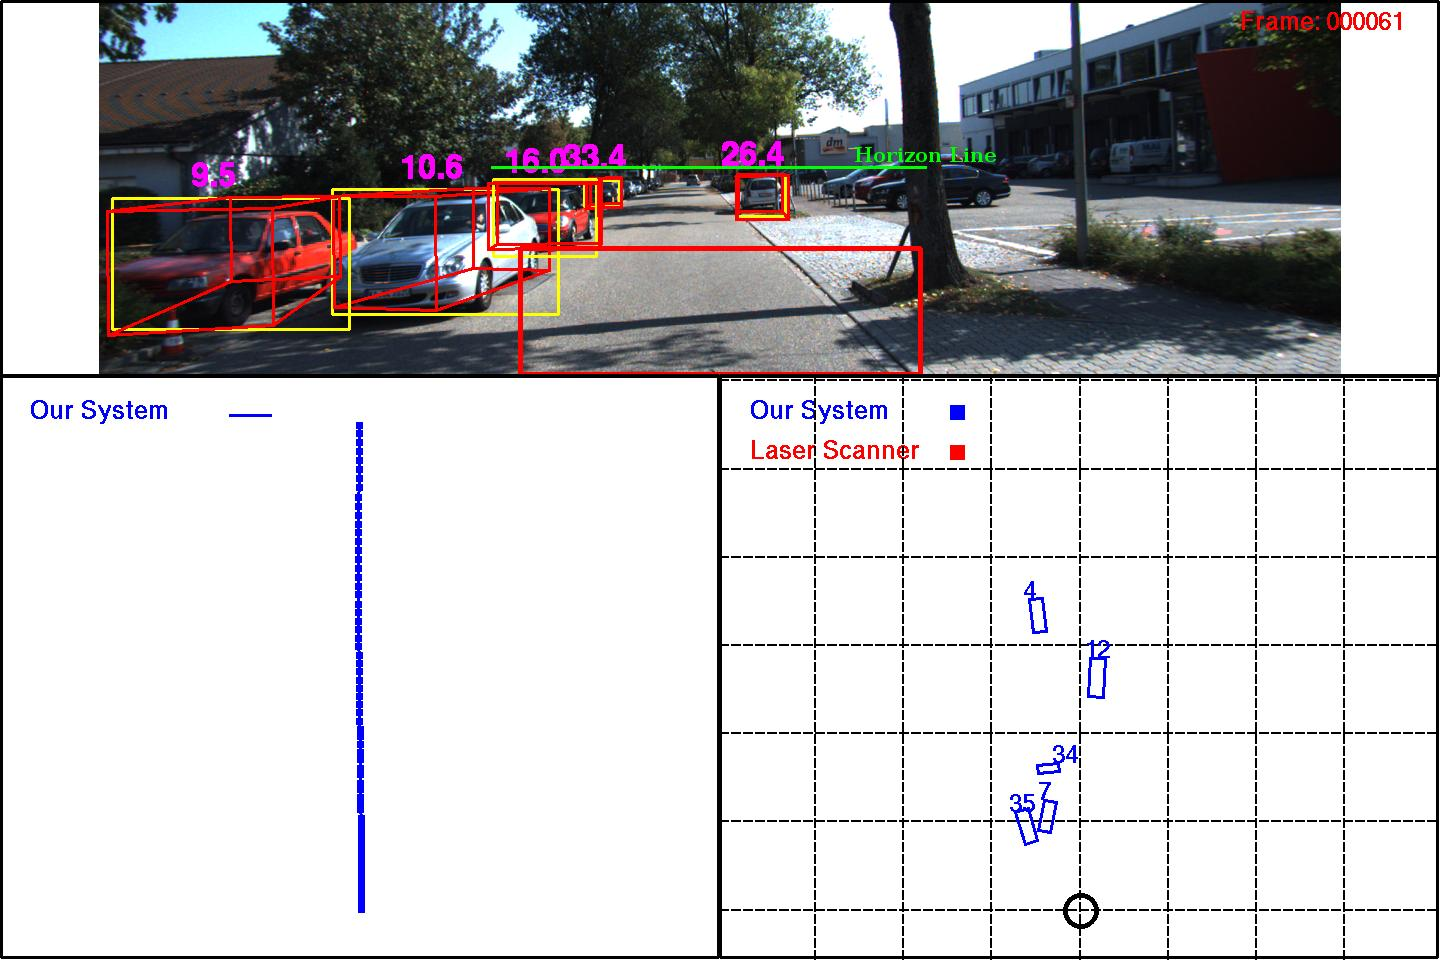
\includegraphics[width=\textwidth]{graphics/Video000061.jpg}
\end{frame}

\begin{frame}
  \frametitle{After}
  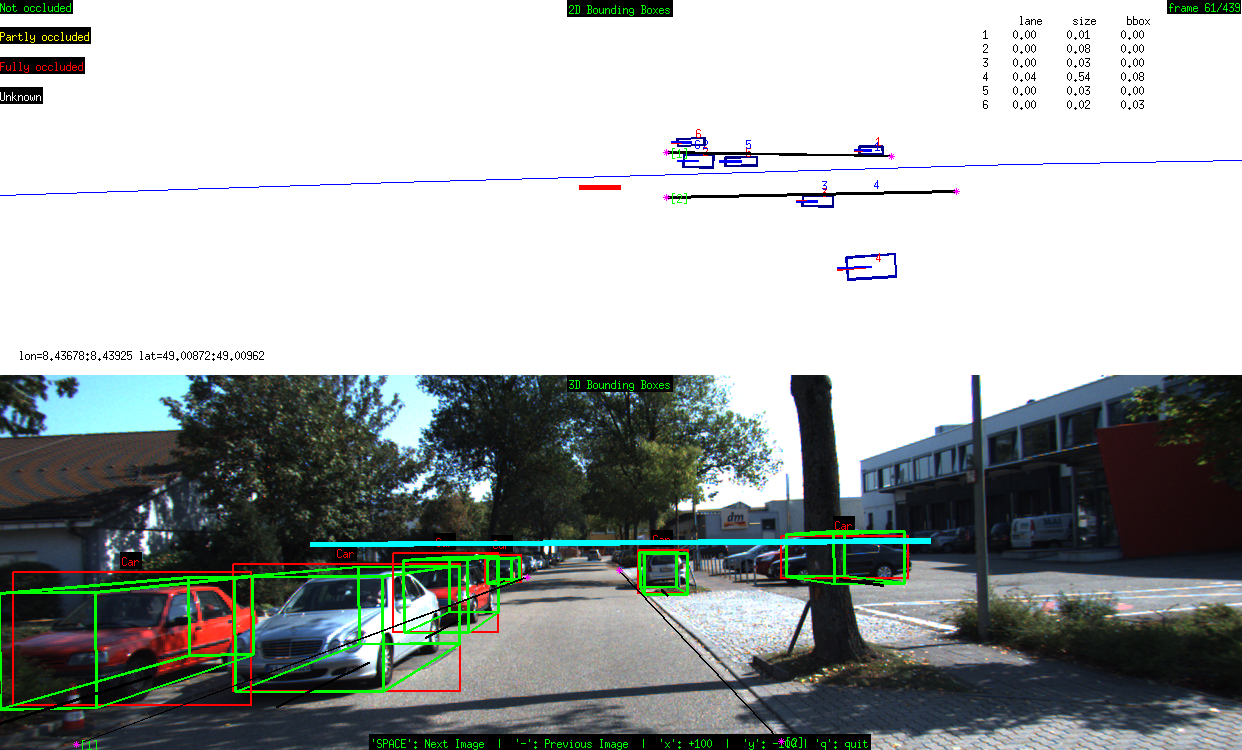
\includegraphics[width=\textwidth]{graphics/61.png}
\end{frame}

\begin{frame}
  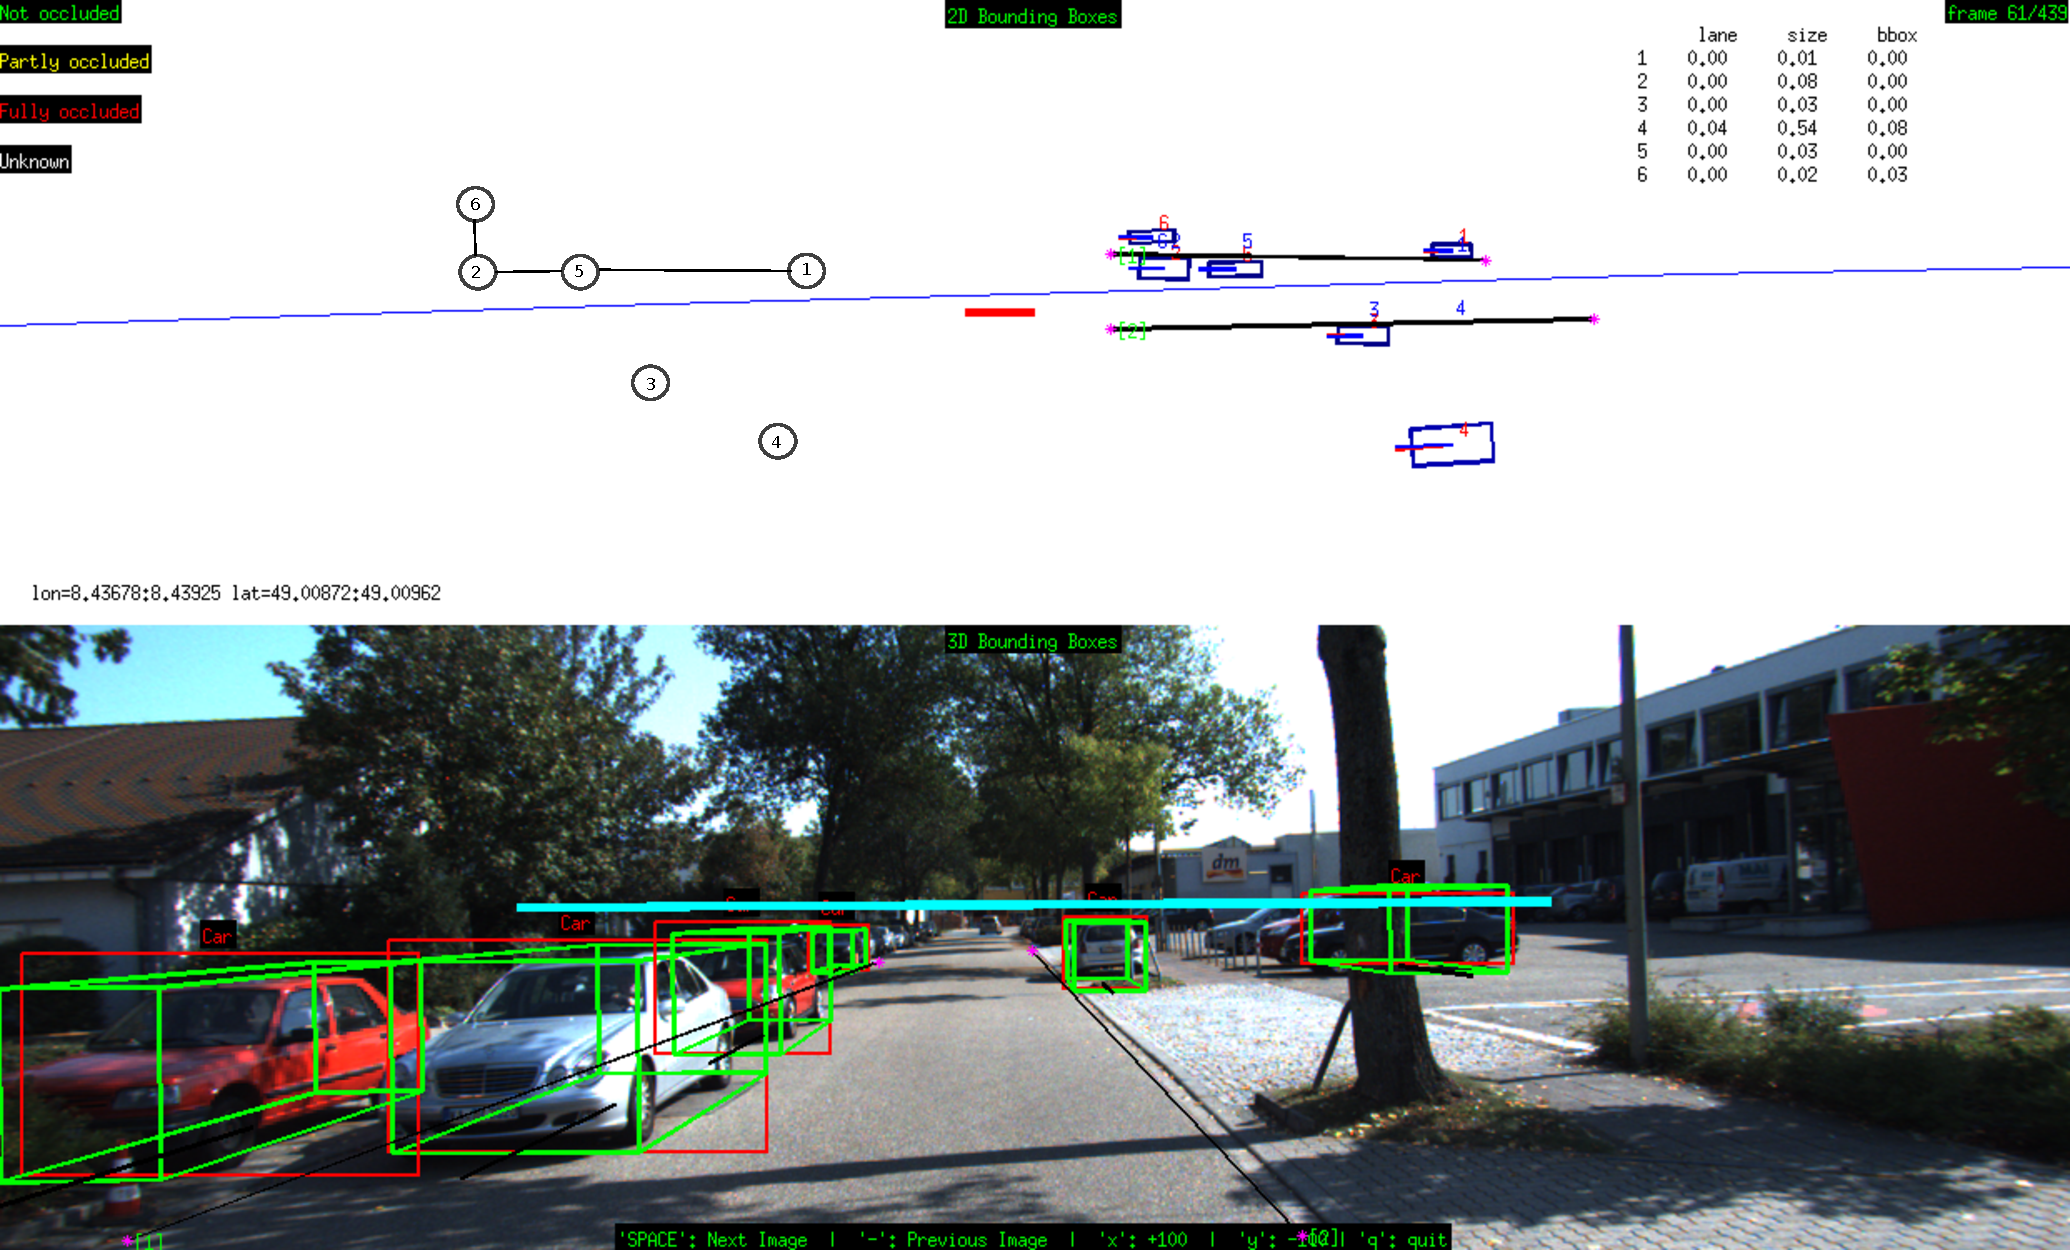
\includegraphics[width=\textwidth]{graphics/61WithGraphicalModel.pdf}
\end{frame}

\begin{frame}
  \centering{
    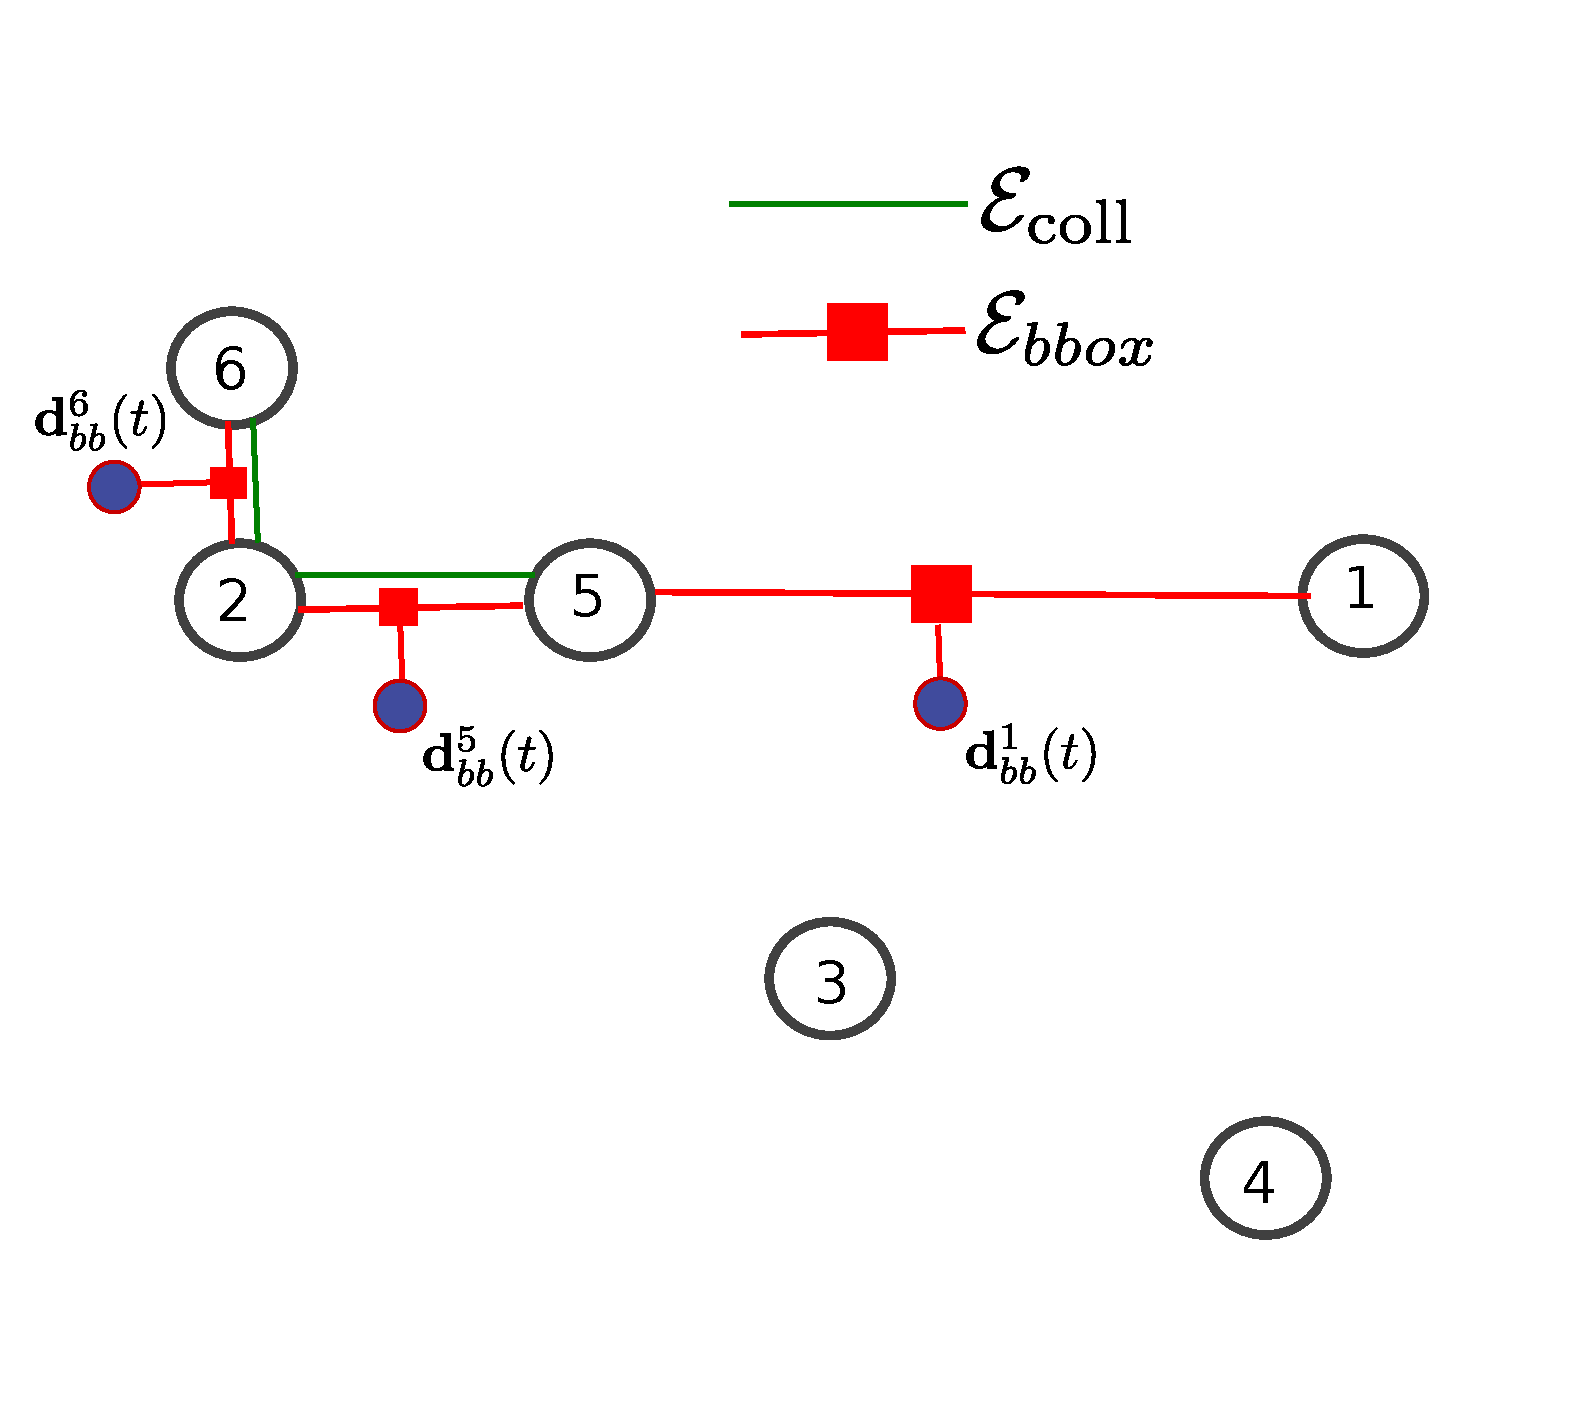
\includegraphics[width=0.5\textwidth]{graphics/graphicalModelFrom61.pdf}
  }
  \pause
  % Collision energy
  %\begin{multline}
  %  \EnergyCol = \frac{1}{1 +
  %\exp(-k(\pos{i}{t}^\top\Sigma_i^{-1}\pos{i}{t})-1)}\\
  %\frac{1}{1 +
  %\exp(-k(\pos{j}{t}^\top\Sigma_j^{-1}\pos{j}{t})-1)}
  %\end{multline}
  %where $k$ is steepness parameter.
  % Bounding box energy occlusion energy

  \begin{align}
    \EnergyCol &=
    \frac{|\Sigma_i|^\frac{1}{4}|\Sigma_j|^\frac{1}{4}}
    {|\frac{1}{2}\Sigma_i + \frac{1}{2}\Sigma_j|^\frac{1}{2}}
    e^{-\frac{1}{8}
      \left(\pos{i}{t} - \pos{i}{t}\right)^\top
      \left(\frac{1}{2}\Sigma_i + \frac{1}{2}\Sigma_j\right)^{-1}
      \left(\pos{i}{t} - \pos{i}{t}\right)
      }
  \end{align}
\end{frame}

\begin{frame}
  \begin{multline}
    \pEnergy{occ}(\relp{i}{t}, \dimsn{i}, \relp{j}{t}, \dimsn{j}) =
               %\sum_{i=1}^N \sum_{t=s_i}^{e_i}
    \sum_kp_{ik}^{\text{track}}(\projectionOf{\dimsn{i}} - \bb{k})^\top \pmb{\rho}(i,j,t)
  \end{multline}
  where $p_{ik}^{\text{track}}$ is the probability of $k$th detection being the
  right track for $i$ hypothesis. (to be computed from tracklet score)
\end{frame}

\begin{frame}
  \centering{
  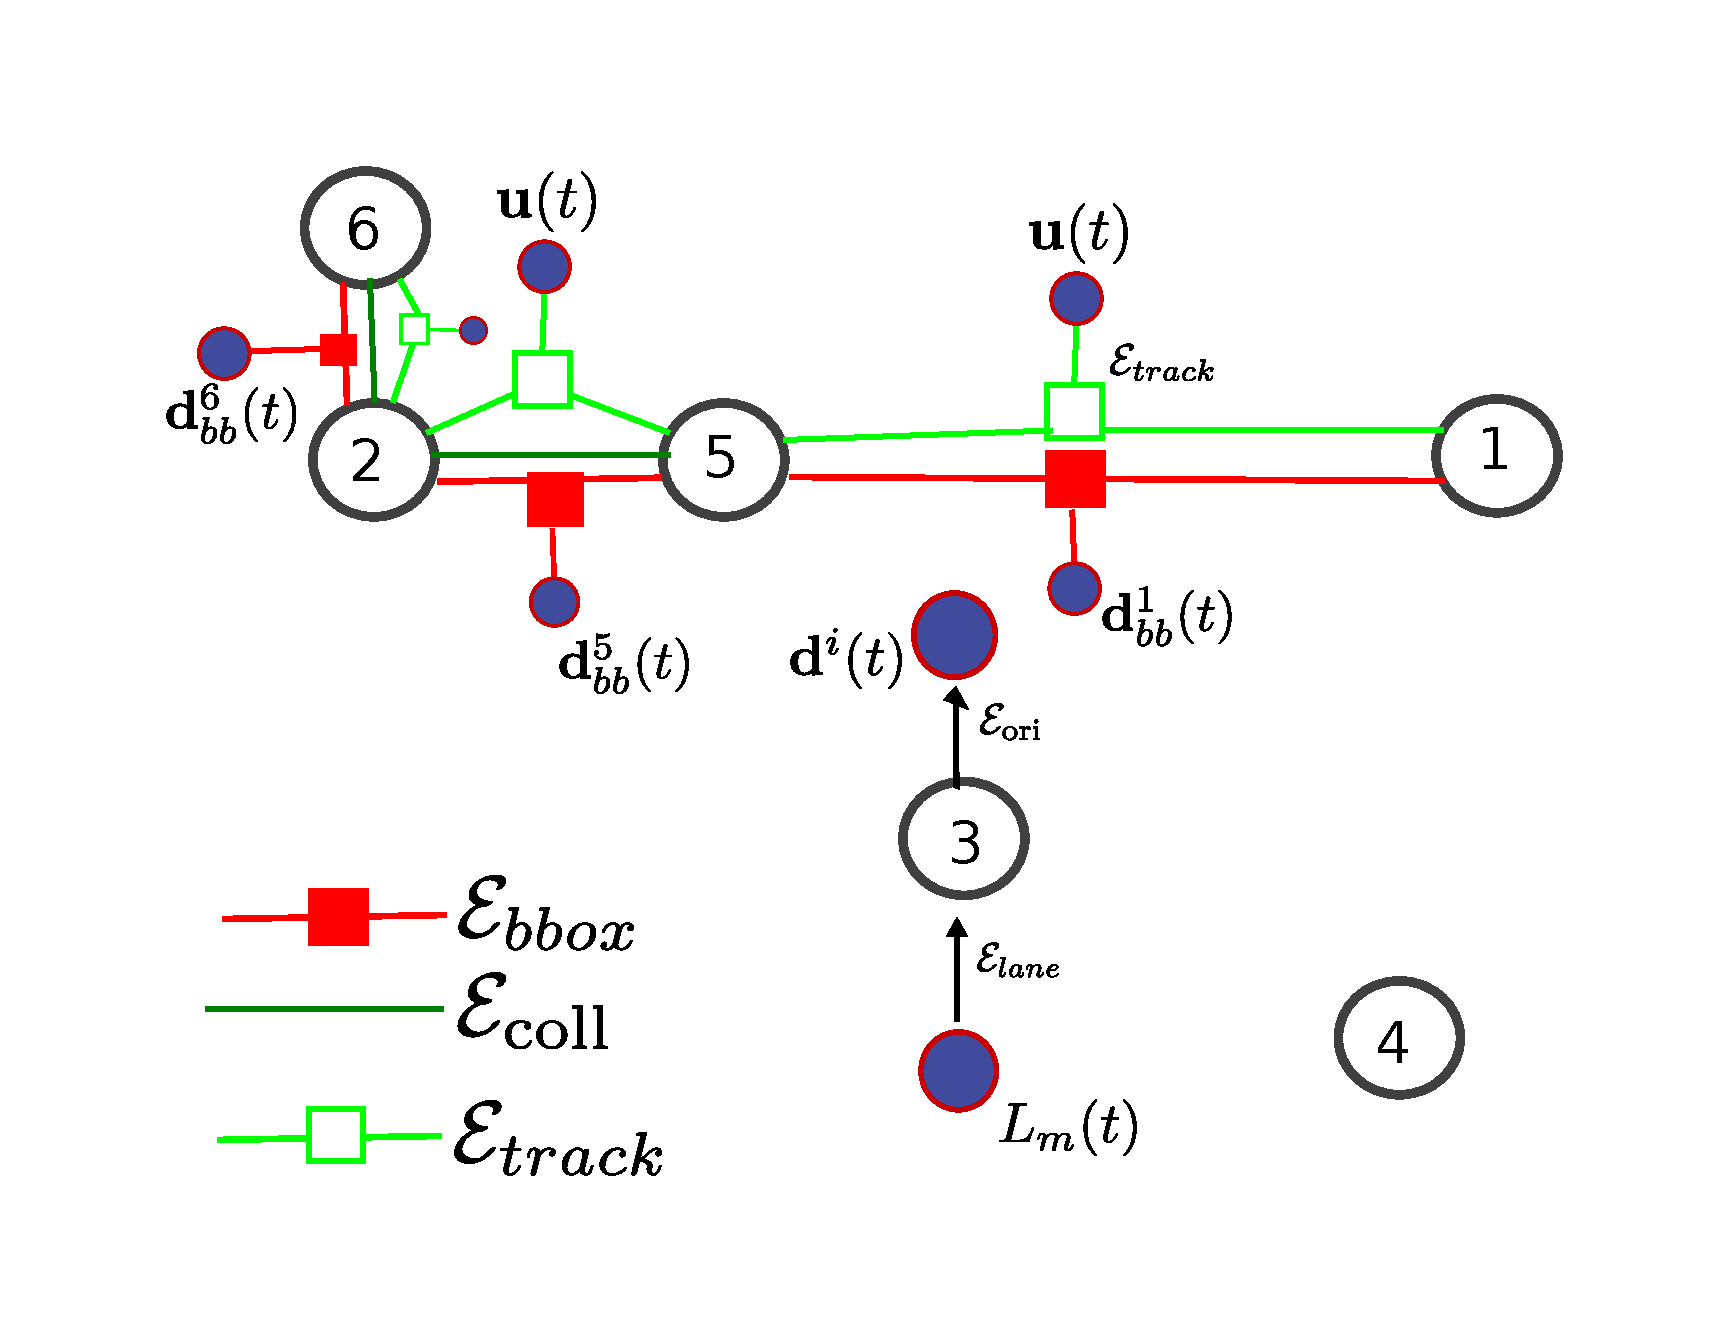
\includegraphics[width=0.5\textwidth]{graphics/graphicalModelFrom61ConstVars.pdf}
}
  \begin{align}
    \Energy{ori} &= 
    %S_t^2(\projectionOf{\dimsn{i}})
    (1 - \cos({\omega}^i_{\text{det}} - \ori{i}{t})
  \end{align}
  \pause
  \begin{multline}
    \Energy{track}(\{ \relp{k}{t} \}_k, \{ \relp{k}{t-1} \}_k, \dimsn{i},
    \dimsn{j}, ) = \\
    \sum_{i=1}^{N} 
    %\sum_{t = s_i}^{e_i}
    \sum_{j = 1}^{M}
    a_j^i(t)\|\trackp{t} - \projectionOf{\invProjectionOf{\trackp{t-1}}}\|^2
  \end{multline}
  where $a_j^i(t)$ is the probability of association of $\trackp{t}$ with
  tracklet $i$.
\end{frame}

\begin{frame}
  $a_j^i(t)$ is soft occlusion dependent probability. Assume the projection of
  tracklet is given by 2D bounding box $[u^i_l, v^i_t, u^i_r, v^i_b] =
\projectionOf{\dimsn{i}}$. Approximate bounding box by ellipse
\begin{align}
\mu_i &= \frac{1}{2}\begin{bmatrix}u^i_l + u^i_r\\v^i_t + v^i_b
\end{bmatrix}\\
\Sigma_i &= \begin{bmatrix} 
\frac{2}{(u^i_l - u^i_r)^2} & 0 \\
0 & \frac{2}{(v^i_t - v^i_b)^2} 
\end{bmatrix}
\end{align}

\end{frame}
\begin{frame}
  \frametitle{The occlusion function}
  Following \cite{milan2013continuous} we model occlusion as soft continuous
  probablistic function that varies with distance from camera and distance of
  the center of projection of the object.
  \begin{align}
    f^i_{\text{occ}}(u, v, \lambda) &= \frac{N(u,v; \mu_i, \Sigma_i)}
    {1 + e^{-\frac{\lambda - \mu^{(d)}_i}{\beta}}}
    \text{where} &\\
    \beta &= \frac{\dimsn{i}_z}{2\log(49)}\\
    \mu_d &= \relp{i}{t}_z
  \end{align}
\end{frame}

\begin{frame}
  Soft occlusion modeling using can be viewed as if the traffic
  participant are being viewed as translucent objects with the probability of
  reflection as $P_{\text{reflection}} = f^i_{\text{occ}}$ . Given a point
  $(u,v)$ on the image, the probability of its association to the $i$ tracklet
  is given by
  \begin{align}
    a^i_j(t) = f^i_{\text{occ}}(u, v, \mu^{(d)}_i)\prod_{k : {\mu^{(d)}_k < \mu^{(d)}_i}}(1 -
    f^k_{\text{occ}}(u, v, \mu^{(d)}_i))
  \end{align}
  where the second term determines the probability of ray being \emph{not
  occluded} by the $k$ objects in front of the $i$th object and the first term
  is the probability of the ray being finally \emph{occluded} by the $i$
  object.
\end{frame}

\begin{frame}
  Since our occlusion function $f^i_{\text{occ}}$ is dependent upon depth as
  well, we can remove the explicit condition over $k:{\mu^{(d)}_k < \mu^{(d)}_i}$.
  \begin{align}
    a^i_j(t) = f^i_{\text{occ}}(u, v, \mu^{(d)}_i)\prod_{k}(1 - f^k_{\text{occ}}(u, v, \mu^{(d)}_i))
  \end{align}
  Also, in practice we compute this association only for the tracklets that
  have overlapping 2D bounding boxes.
  \begin{align}
    a^i_j(t) &= \begin{cases}
    f^i_{\text{occ}}
    \prod\limits_{k : (u,v) \in \projectionOfi{k}{\dimsn{k}}}
    (1 - f^k_{\text{occ}})
    & \text{if } i : (u,v) \in \projectionOf{\dimsn{i}} \\
    0 & \text{otherwise}
    \end{cases}
  \end{align}
\end{frame}


\begin{frame}
  \centering{
  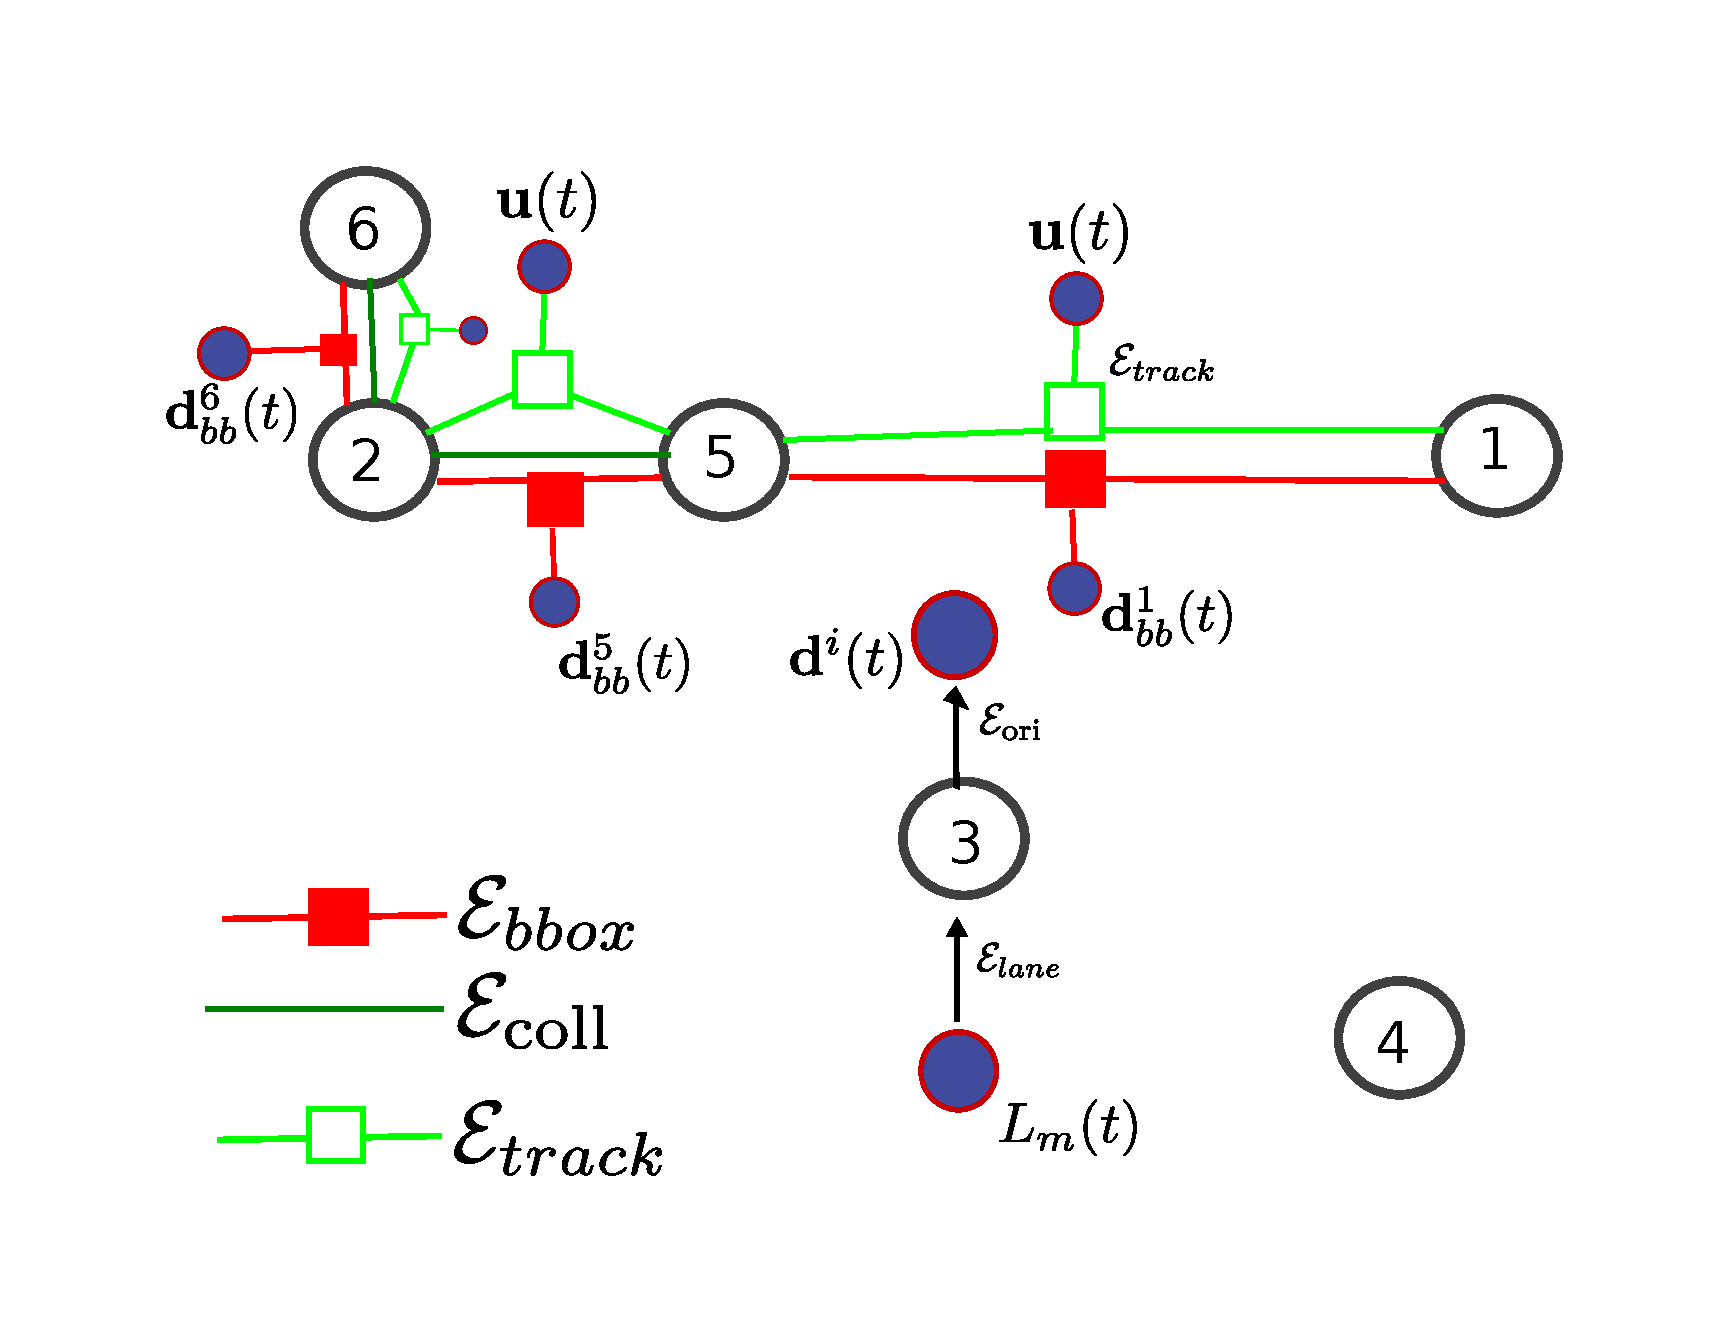
\includegraphics[width=0.5\textwidth]{graphics/graphicalModelFrom61ConstVars.pdf}
}

  \begin{align}
    \Energy{lane} &= 
    \sum_{m : \text{DIST}(L_{m}(k), \pos{i}{t}) < 50}\frac{1 - \ori{i}{t} \cdot \text{TAN}(L_{m}(k),
    \pos{i}{t}) }
    {1 + exp(-q(w_{\text{road}} - \text{DIST}(L_{m}(k), \pos{i}{t})))}
  \end{align}
\end{frame}

\begin{frame}
  \centering{
  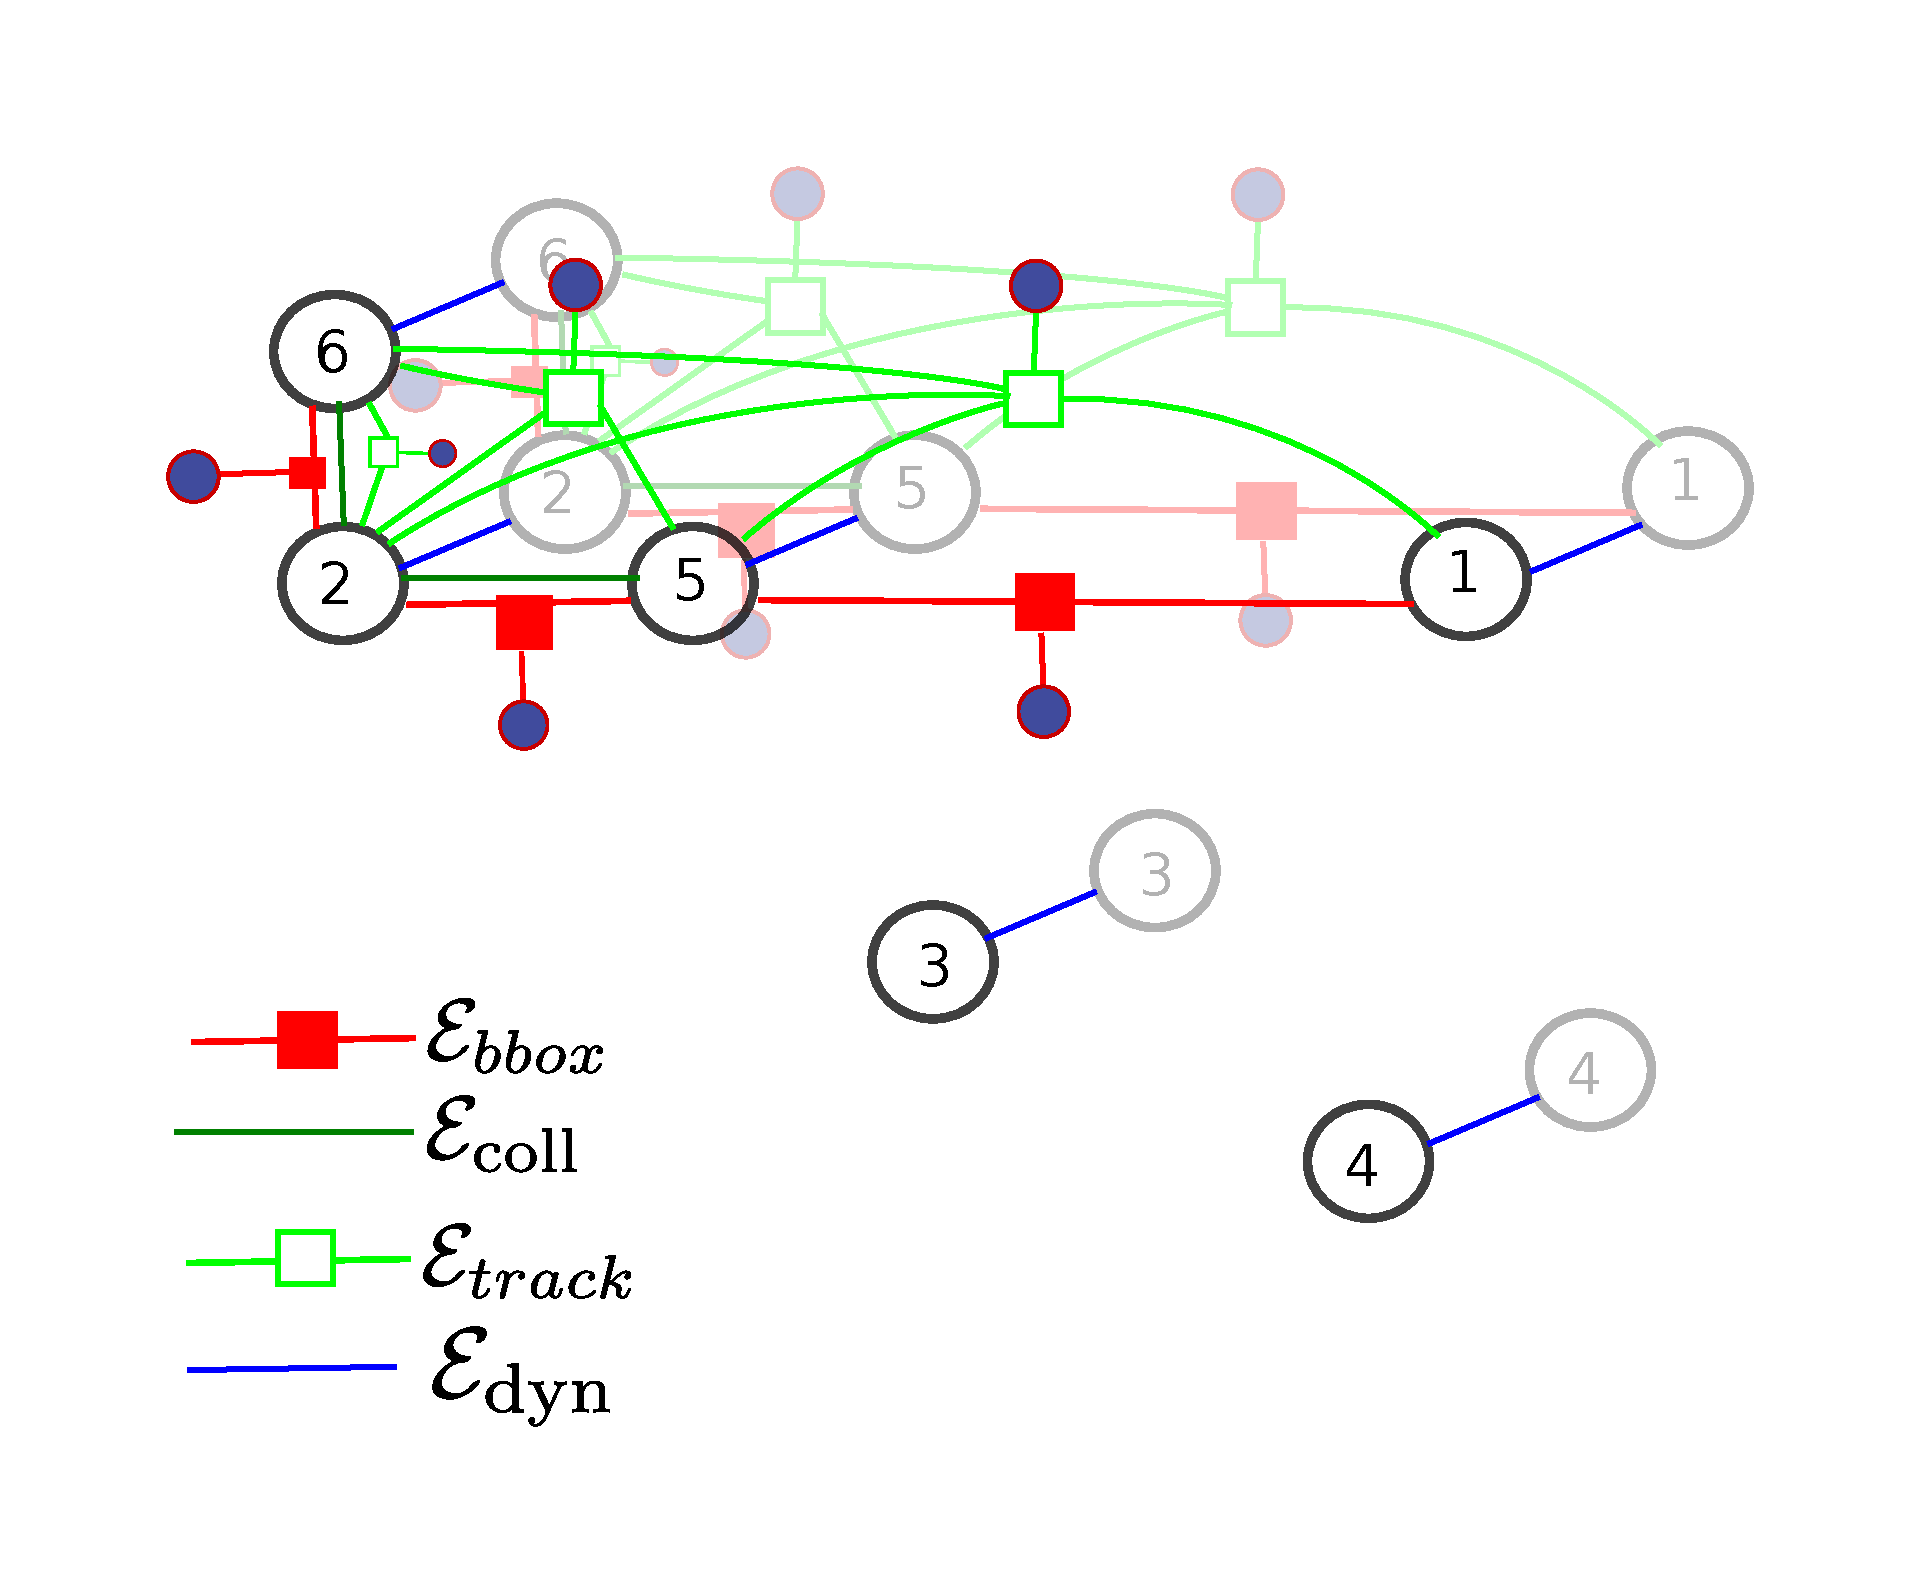
\includegraphics[width=0.6\textwidth]{graphics/graphicalModelFrom61withConstNodes.pdf}
}
\begin{align}
  \Energy{dyn-hol} &= 1 - \ori{i}{t-1} \cdot (\pos{i}{t} - \pos{i}{t-1})\\
  \Energy{dyn-ori} &= \|\ori{i}{t} - \ori{i}{t-1}\|^2\\
  \Energy{dyn-vel} &= \|(\pos{i}{t} - 2\pos{i}{t-1}) + \pos{i}{t-2}\|^2
\end{align}
\end{frame}

\begin{frame}
  \frametitle{Inference}
  \begin{itemize}
    \item Most previous works use MCMC which is slow
      \pause
    \item The number of edges $\approx$ 10-20 per frame $\approx$ 500-1000 for
      50 frame sequence
      \pause
    \item The described graph is mostly trees with a few loops
      \pause
    \item Variants of Belief propagation with damping seems a good bet.
      \pause
    \item However, traditional version of inference algorithms including BP,
      TRW-S, Dual decomposition discrete state space.
      \pause
    \item We will need simpler smooth analytical approximation of messages for
      continuous state spaces.
      \pause
    \item The approximation will need to be done for each message passing step
  \end{itemize}
\end{frame}



\begin{frame}
\begin{center}
\begin{tikzpicture}
  \node (img1) {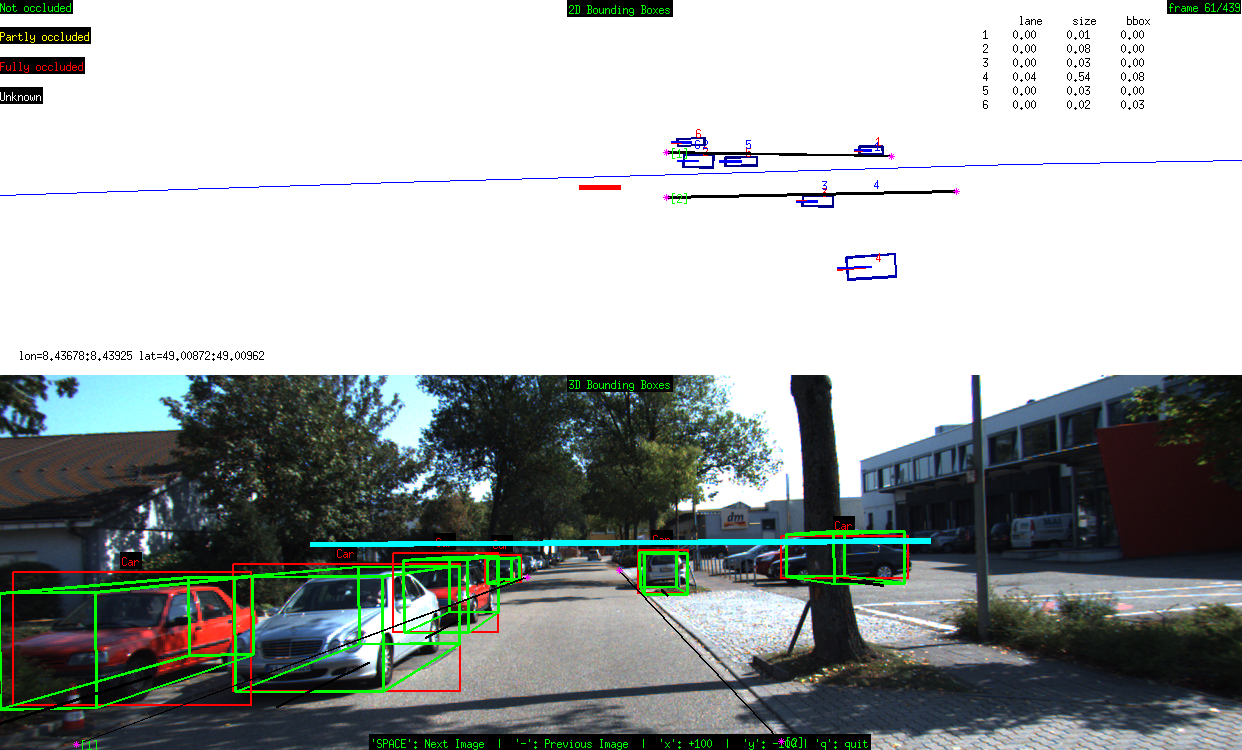
\includegraphics[width=\textwidth]{graphics/61.png}};
  \node (img2) at (-2.5, 1.8) {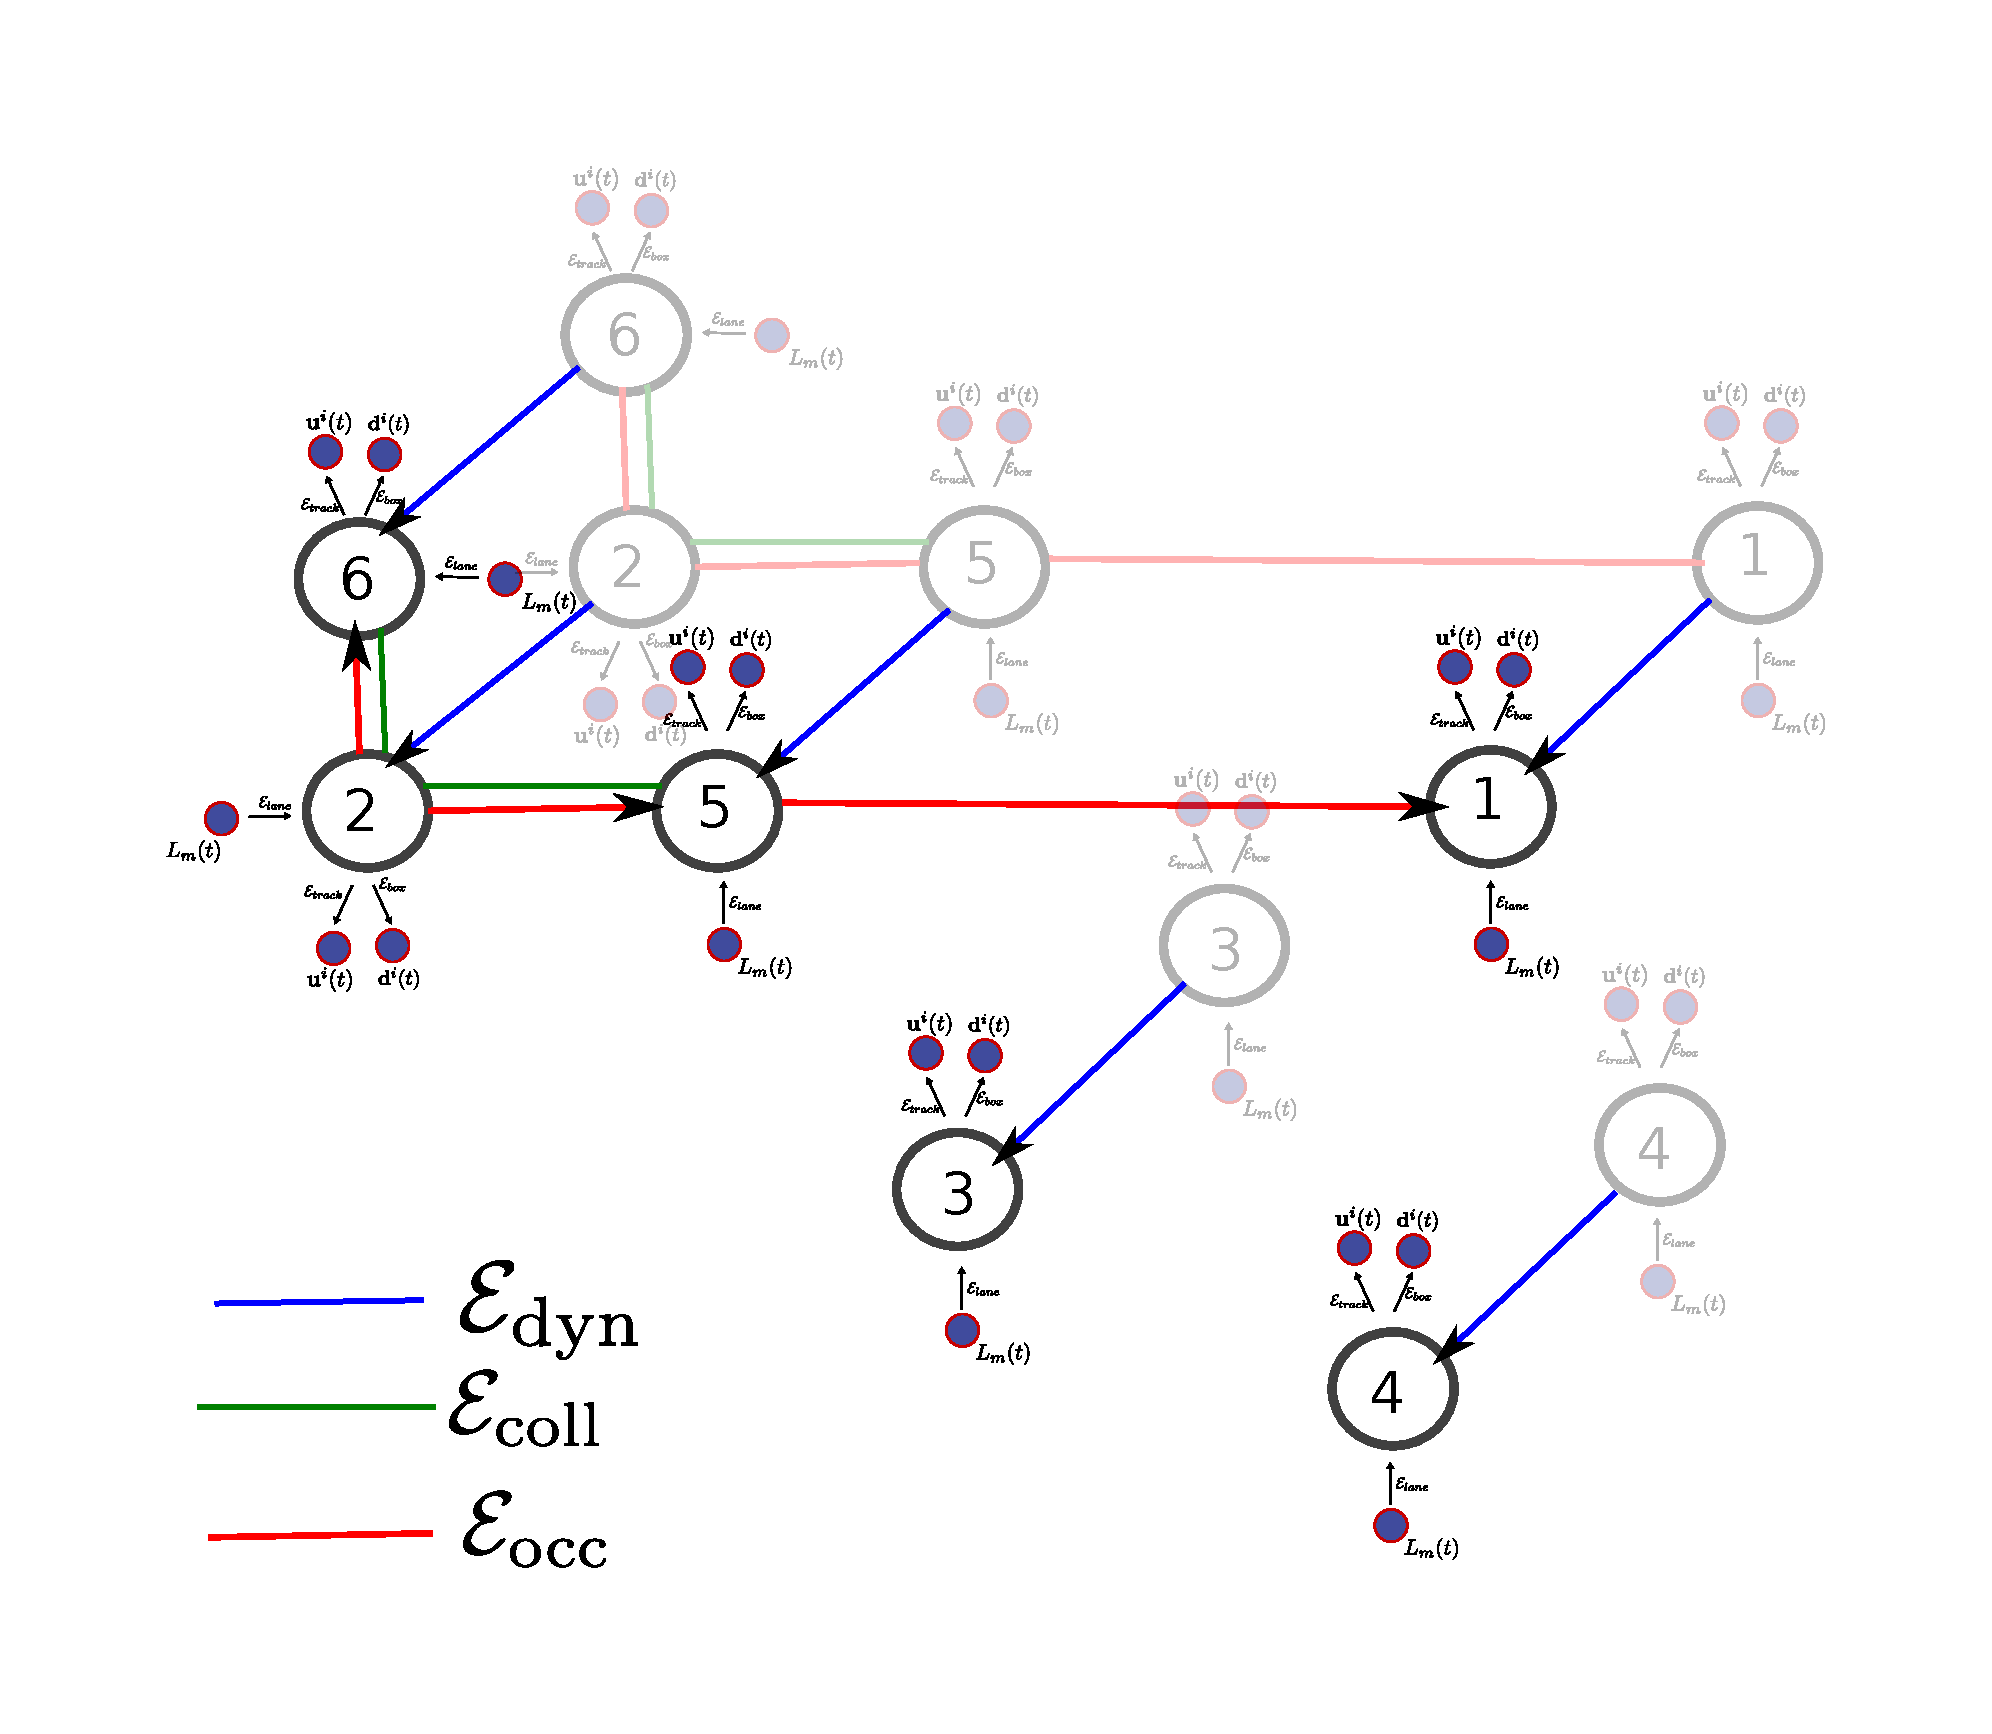
\includegraphics[height=0.3\textwidth]{graphics/graphicalModelFrom61withConstNodesDirections.pdf}};
\end{tikzpicture}
\end{center}
\end{frame}

\bibliographystyle{plannat}
\bibliography{model}
\end{document}
